\section{Regularización}

La última técnica a usar en este texto es la técnica de regularización, esta es usada para librarnos de dos problemas al momento de entrenar. Estos problemas son el \textit{sobre ajuste} y el \textit{ajuste pobre}, en inglés \emph{overfitting} y \emph{underfitting} respectivamente.

Recordemos que dado un problema de aprendizaje, se define un espacio de hipótesis, es decir, una familia de posibles funciones que vamos a utilizar para encontrar la función objetivo, que queremos aproximar. 

El espacio de hipótesis puede ser tan grande o tan pequeño como la cantidad de funciones que estén contenidas en él. Así tenemos dos situaciones:
\begin{itemize}
 \item Si el espacio de hipótesis, no contiene a la función objetivo, entonces por más que ejecutemos los algoritmos de entrenamiento, no va a ser posible llegar a una buena aproximación.
 \begin{example}
  Si la función objetivo tiene la forma de una parábola, y únicamente la intentamos aproximar con funciones lineales, es claro que nunca vamos a dar una buena aproximación.
 \end{example}

 \item Si el espacio de hipótesis, es demasiado gigantesco, podemos llegar a tener problemas encontrando la respuesta correcta. 
\end{itemize}

Las dos situaciones anteriores nos llevan a los dos problemas antes mencionados:
\begin{description}
 \item [Ajuste pobre] 
 Cuando un modelo, no logra reducir suficientemente el error sobre el conjunto de entrenamiento (menos aún sobre el de validación) ver \fref{fig:underF}.
  \begin{figure}[H]
   \centering
   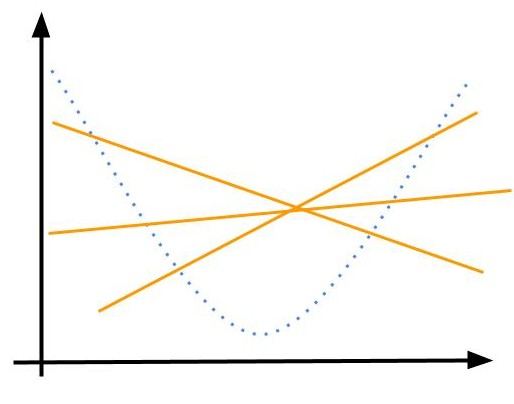
\includegraphics[scale=0.5]{../Figuras/underfitting.jpg}
   \caption{Ejemplo de ajuste pobre. La línea punteada es la función objetivo, las líneas naranjas el espacio de hipótesis.}
   \label{fig:underF}
  \end{figure}

 \item [Sobre ajuste]
 Cuando un modelo, reduce muy bien el error con el conjunto de entrenamiento, pero con el conjunto de validación el error es muy alto, es decir, la hipótesis no generaliza a datos no vistos previamente, ver \fref{fig:overF}.
 \begin{example}
  Los datos del entrenamiento asemejan la función de un polinomio, entonces la red aprende solo a identificar los datos que pasen por la función, al momento de agregar datos nuevos estos probablemente nos se comporten conforme al polinomio y nunca los clasifique adecuadamente. 
 \end{example}

  \begin{figure}[H]
   \centering
   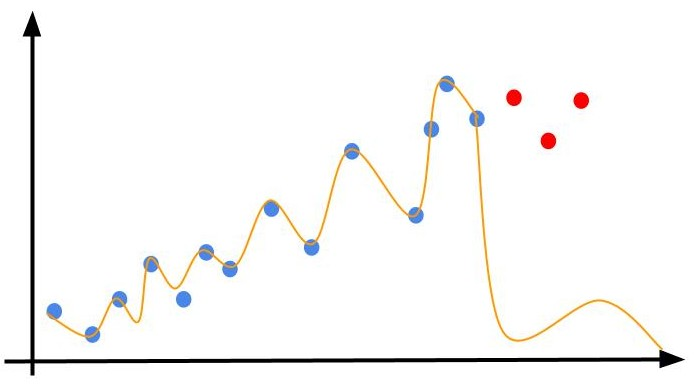
\includegraphics[scale=0.5]{../Figuras/overfitting.jpg}
   \caption{Ejemplo de sobre ajuste. La función aproximada de color naranja. Los datos durante el entrenamiento de color azul. Los datos nuevos de color rojo.}
  \label{fig:overF}
  \end{figure}
 \end{description}

Estos dos problemas puden suceder por dos razones distintas:
\begin{enumerate}
 \item La cantidad de neuronas, dos casos:
    \begin{itemize}
     \item \textbf{Faltan neuronas}: El espacio de hipótesis es muy simple para poder aproximar la función, es decir, tenemos un \textit{ajuste pobre}.
    
    \item \textbf{Sobran neuronas}: El espacio de hipótesis es muy expresivo. No obtiene las características de la función objetivo, sino que memorizó las etiquetas de los datos de entrada, es decir, tenemos un \textit{sobreajuste}.
    \end{itemize}

 \item Faltan datos de entrenamiento, entonces independientemente del número de neuronas, el error en los datos de validación no baja, o incluso ni en los datos del entrenamiento.
\end{enumerate}

Cuando nos sobran nueronas lo podemos detectar, porque al reducir neuronas, el desempeño de la red entrenada en el conjunto de entrenamineto, no empeora significativamente, y el desempeño con los datos de validación mejora.

Para automatizar la búsqueda en un espacio de hipótesis lo suficientemente expresiva vamos a usar la regularización.

Lo que vamos a hacer es modificar la función de pérdida, la nueva función va a estar integrada por dos componentes; la función de error (que ya teníamos), y un  término de penalización sobre las magnitudes de los pesos de la red. Considerando estas dos anteriores,  la función que estamos tratando de minimizar es  la suma de esas dos.

El mínimo de esta función hallará un punto de compromiso tal que:
\begin{itemize}
 \item reduce el error lo más posible
 \item solo crecen aquellos pesos que contribuyen mejor a reducir el error, compensando por la contribución de su magnitud creciente.
\end{itemize}

Es decir ahora tenemos una red en la cual colocamos desde el inicio muchas neuronas, lo cual tendería a producir un sobre ajuste. Lo que vamos a hacer es, penalizar los pesos de manera que el algoritmo de optimización haga que solamente aquellas conexiones que realmente están contribuyendo a reducir el error, tengan magnitudes significativas. Aquellas conexiones que no contribuyan entenderán a tener magnitudes muy pequeñas, casi como si no estuvieran ahí. El algoritmo de optimización hara que algunas de las conexiones queden muy débiles y básicamente ya no contribuyan. Entonces la hipótesis que se va a aprender va a ser más sencilla.

Dependiendo de qué tan rigurosos seamos con la penalización podemos hacer que, las únicas conexiones que pueden subir su magnitud en realidad sean muy pocas. También podría darse el problema de ajuste pobre, se  tiene que ajustar bien el termino de penalización que lo vamos a denotar como \emph{$\lambda$}.

La función de perdida se va actualizar de la siguiente forma:
\begin{equation}
 J(\Theta) = Error(\Theta)+\dfrac{\lambda}{2m}\sum_{\Theta}\theta^2
 \label{eq:errorR}
\end{equation}

\begin{equation}
 \nabla_{\theta}J^{(l)} = \nabla Error_{\Theta}^{(l)}+\dfrac{\lambda}{m}\left[ \right]
\end{equation}
%\begin{bmatrix} 0 \\ \Theta_{[:,1:]} \end{bmatrix}

Entonces vamos a tener una gráfica parecida a la siguiente:
  \begin{figure}[H]
   \centering
   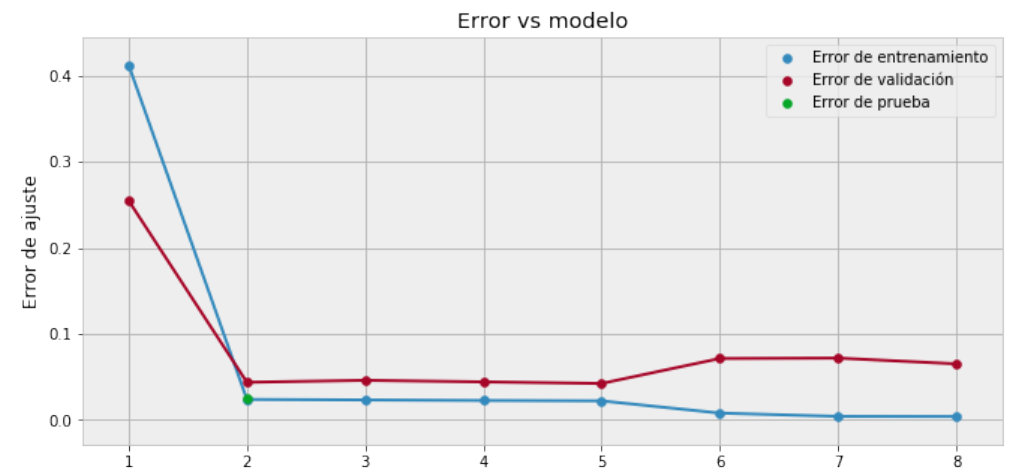
\includegraphics[width=\textwidth ]{../Figuras/graficaOO.png}
   \caption{Sobreajuste.}
  \label{fig:grafica00}
  \end{figure}

 En la ecuación \ref{eq:errorR} que del lado izquierdo tenemos nuestra función de error (podría ser una entropía cruzada, diferencias cuadrado), el segundo término es la penalización, la más común es  sumar los todos los cuadrados de las magnitudes, de todos los pesos que tienen la red, este término va a provocar que la función suba de valor, si estamos utilizando pesos con magnitudes grandes. 
 
 La manera de minimizar los valores, es dejar subir solamente los valores de aquellos pesos que ayuden a compensar, bajando la penalización. La penalización está regida por el parámetro lambda, entre más grande sea lambda, se observa en la \fref{fig:grafica00} que se incrementa el valor de esta función, por culpa de los pesos. Entonces, si la lambda es muy pequeña el término dominante va a ser la función original de error y poca penalización por tanto muy poco efecto, por el hecho de haberle subido la magnitud de los pesos, vamos a obtener un sobreajuste. Esto equivaldría a tener nuestra red neuronal con el montón de neuronas que le pusimos, no hay penalización y podríamos tender precisamente al problema del sobreajuste. 
 
 Entonces vaemos el lado derecho de la gráfica \fref{fig:grafica00}. El error en el entrenamiento se esta penalizando tanto por los pesos que el algoritmo de optimización, minimizo los pesos y casi no corregio el error, entonces tenemos un ajuste pobre. En ese caso  nuestra red  no está modelando bien nuestra función, tenemos un error bastante alto y la función de validación también está creciendo. 
 
 En el la parte de en medio de la gráfica \fref{fig:grafica00} es donde de obtiene el equilibrio, entre la cantidad de neuronas adecudas y la cantidad de pesos significativos, que nos va a minimizar o eliminar el problema de un pobre o un sobre ajuste.
 
 \subsection{Dropout}
 
 Otra estrategia para regularizar es la deserción o descarte de algunas neuronas(\emph{dropout} en inglés). 
 Durante el entrenamiento, una cierta cantidad de salidas de capas ocultas se ignoran \emph{aleatoriamente} (se les da valor final de 0) con probabilidad $1-p$, es decir algunas neuronas de las capas ocultas se activan con un probablidad $p$. 

 En esta técnica no se modifica la función de error, si no se modifica propiamente la red, ver \fref{fig:dropout}. En cada epoca, durante el entrenamiento se puede volver a elegir las neuronas a descartar, o no. 
 La capa alterará su conectividad y buscará caminos alternativos para transmitir la información en la siguiente capa. Como resultado, cada actualización de una capa durante el entrenamiento se realiza con una configuración diferente de la capa. Así se puede simular el entrenamiento de una gran cantidad de redes neuronales con diferentes arquitecturas en paralelo.

  \begin{figure}[h]
   \centering
   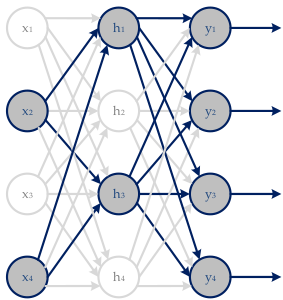
\includegraphics[scale=.5]{../Figuras/dropout.png}
   \caption{Dropout (desarrollado por Geoffrey Hinton y sus estudiantes en la Universidad de Toronto).}
  \label{fig:dropout}
  \end{figure}

 Al momento de pasar los datos de prueba, todas las neuronas están activas. Pero se han reducido en p, esto sucede porque después de la eliminación en el entrenamiento, las siguientes capas recibirán valores más bajos. Sin embargo, en la fase de prueba, mantendremos todas las unidades, por lo que los valores serán mucho más altos de lo esperado, es por eso que necesitamos reducirlos, por un facto igual a la tasa de deserción p, para equilibrar el hecho de que hay más unidades activas que en tiempo de entrenamiento. Para información del tema puede leer el capítulo cuatro, sección 4.4.3 Adding dropout, Deep Learning With Python, 2017.  
 
 

